% ft-12-Optimization.tex

\documentclass[xcolor=dvipsnames]{beamer}

\usepackage{cancel}
\renewcommand{\CancelColor}{\color{red}}
\usepackage{graphicx}
\usepackage{wrapfig}
\usepackage{colortbl}
\usepackage{color}
\usepackage{alltt}
\renewcommand*{\thefootnote}{\fnsymbol{footnote}}
\definecolor{myblue}{rgb}{0.8,0.85,1}

\mode<presentation>
{
  \usetheme{Warsaw}
  \setbeamercovered{transparent}
}
% \usecolortheme[named=OliveGreen]{structure}
\setbeamertemplate{navigation symbols}{} 
\setbeamertemplate{blocks}[rounded][shadow=true] 

% this is for overlaying math symbols, see https://tex.stackexchange.com/questions/12895/overlay-symbol-with-another
\def\qeq{\mathrel{%
    \mathchoice{\QEQ}{\QEQ}{\scriptsize\QEQ}{\tiny\QEQ}%
}}
\def\QEQ{{%
    \setbox0\hbox{$\longrightarrow$}%
    \rlap{\hbox to \wd0{\hss/\hss}}\box0
  }}

\newcounter{expls}
\setcounter{expls}{0}
\newcommand{\beispiel}[1]{\refstepcounter{expls}\textbf{Example \arabic{expls}: #1.}}

\newcounter{exercise}
\setcounter{exercise}{0}
\newcommand{\ubung}[0]{\refstepcounter{exercise}\textbf{Exercise \arabic{exercise}: }}

\newif\ifBCITCourse
\BCITCoursetrue
% \BCITCoursefalse
\newif\ifWhichCourse
\WhichCoursetrue
% \WhichCoursefalse
\ifBCITCourse
\ifWhichCourse
\newcommand{\CourseName}{Technical Mathematics for Food Technology}
\newcommand{\CourseNumber}{MATH 1441}
\newcommand{\CourseInst}{BCIT}
\else
\newcommand{\CourseName}{Technical Mathematics for Geomatics}
\newcommand{\CourseNumber}{MATH 1511}
\newcommand{\CourseInst}{BCIT}
\fi
\else
\newcommand{\CourseName}{Philosophy and Literature}
\newcommand{\CourseNumber}{PHIL 375}
\newcommand{\CourseInst}{UBC}
\fi

\title{Chain Rule}
\subtitle{{\CourseNumber}, BCIT}

\author{\CourseName}

\date{November 16, 2017}

\begin{document}

\begin{frame}
  \titlepage
\end{frame}

\begin{frame}
  \frametitle{Relative Extrema}
A function $f$ has a \alert{relative maximum} at $x=c$ if there exists
an open interval $(a,b)$ containing $c$ such that $f(x)\leq{}f(c)$ for
all $x$ in $(a,b)$.

\bigskip

A function $f$ has a \alert{relative minimum} at $x=c$ if there exists
an open interval $(a,b)$ containing $c$ such that $f(x)\geq{}f(c)$ for
all $x$ in $(a,b)$.
\end{frame}

\begin{frame}
  \frametitle{Derivatives and Extrema}
  At any number $c$ where a differentiable function $f$ has a relative
  extremum, $f'(c)=0$. The converse is not true. Consider the
  following two functions and their derivatives.
\begin{equation}
  \label{eq:thapoich}
f_{1}(x)=x^{3}+x^{2}-5x-1
\end{equation}
\begin{equation}
  \label{eq:gohshaem}
f_{2}(x)=\left(\frac{3}{10}x\right)^{3}
\end{equation}
\end{frame}

\begin{frame}
  \frametitle{Derivatives and Extrema Graph I}
  \begin{figure}[h]
    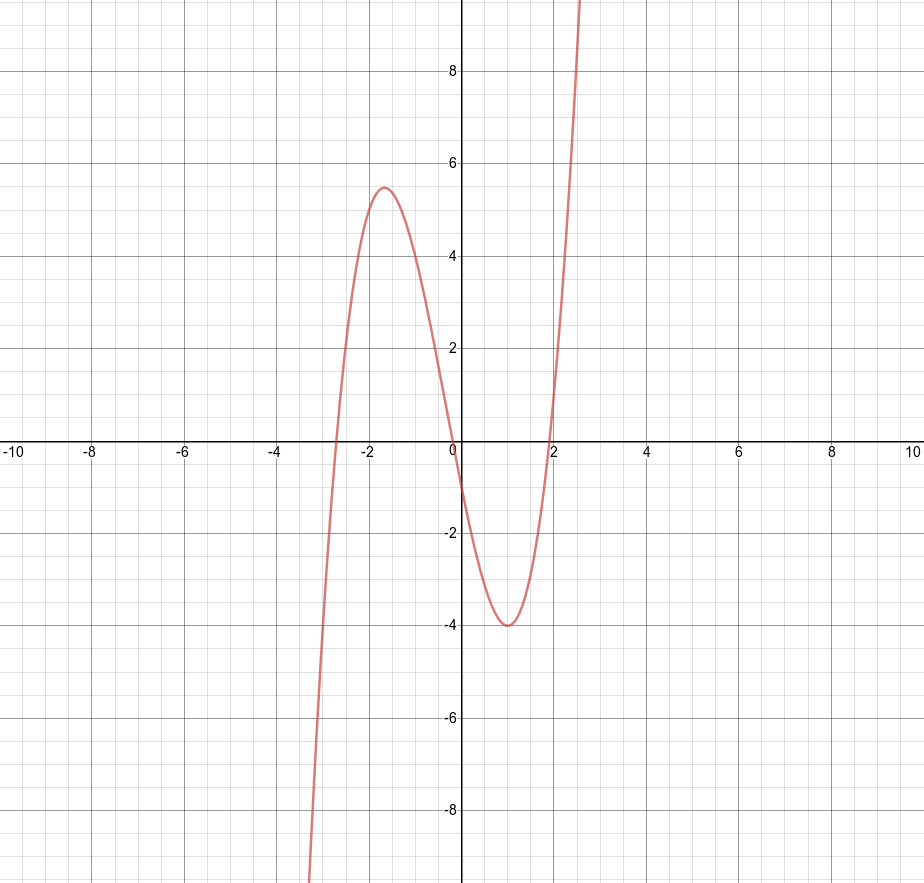
\includegraphics[scale=.3]{./extrema1.png}
  \end{figure}
\end{frame}

\begin{frame}
  \frametitle{Derivatives and Extrema Graph II}
  \begin{figure}[h]
    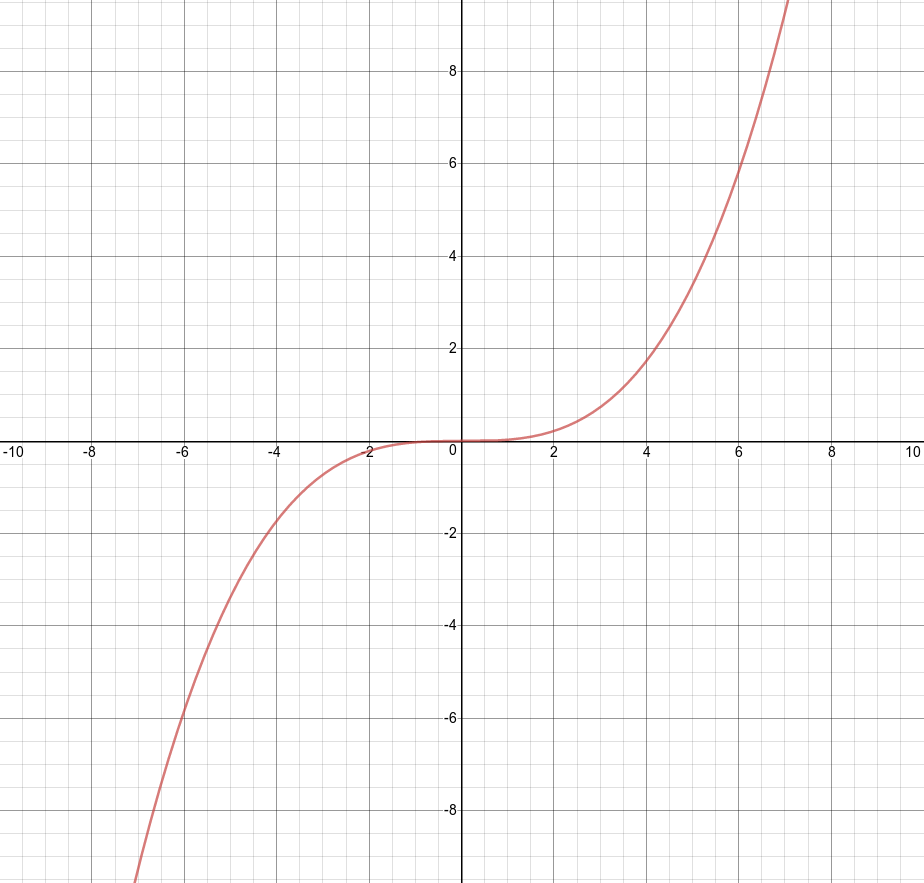
\includegraphics[scale=.3]{./extrema2.png}
  \end{figure}
\end{frame}

\begin{frame}
  \frametitle{Derivatives and Extrema Caution}
Note that a function may have an extremum at a point where the
derivative is not $0$ if at that point the function is not
differentiable. Consider this function and its derivative.
\begin{equation}
  \label{eq:ceezukoh}
f_{3}(x)=x^{\frac{2}{3}}
\end{equation}
\begin{block}{Critical Number}
  A \alert{critical number} of a function $f$ is any number $x$ in the
  domain of $f$ such that $f'(x)=0$ or $f'(x)$ does not exist.
\end{block}
\end{frame}

\begin{frame}
  \frametitle{Derivatives and Extrema Graph III}
  \begin{figure}[h]
    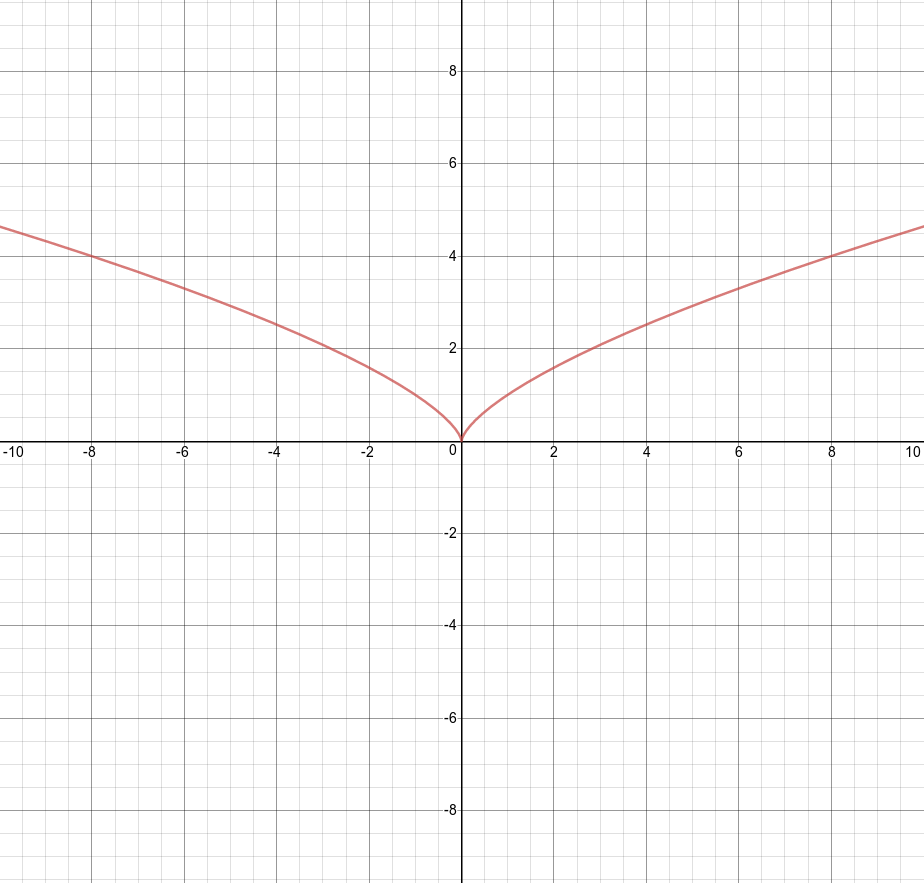
\includegraphics[scale=.3]{./extrema3.png}
  \end{figure}
\end{frame}

\begin{frame}
  \frametitle{Extrema Exercises}
Find the relative maxima and relative minima, if any, of each
function.
\begin{equation}
  \label{eq:xoongohh}
f(x)=x^{3}-4x
\end{equation}
\begin{equation}
  \label{eq:aghuomoh}
h(t)=-t^{2}+6t+6
\end{equation}
\begin{equation}
  \label{eq:yakovuap}
f(x)=\frac{1}{2}x^{4}-x^{2}
\end{equation}
\begin{equation}
  \label{eq:aweefahx}
g(x)=\frac{x+1}{x}
\end{equation}
\begin{equation}
  \label{eq:ebukatio}
f(x)=x\sqrt{x-4}
\end{equation}
\begin{equation}
  \label{eq:inaidimo}
h(s)=s^{\frac{5}{3}}
\end{equation}
\end{frame}

\begin{frame}
  \frametitle{Analyzing Functions}
To analyze a function, determine the following features:
\begin{itemize}
\item Domain and range of the function.
\item Zeros (also called $x$-intercepts) of the function.
\item Critical points, maxima, minima.
\item Inflection points.
\item Asymptotes.
\item Is the function even ($f_{1}(x)=x^{2}+1$) or odd ($f_{2}(x)=x^{3}-x$)?
\end{itemize}
\end{frame}

\begin{frame}
  \frametitle{Analyzing Functions Exercises}
Analyze the following functions:
\begin{equation}
  \label{eq:ohkaedoy}
g_{1}(x)=-x^{2}+3x
\end{equation}
\begin{equation}
  \label{eq:teecakie}
g_{2}(x)=3x^{\frac{2}{3}}-2x
\end{equation}
\begin{equation}
  \label{eq:saepaego}
g_{3}(x)=\frac{2t^{2}}{t^{2}+3}
\end{equation}
\begin{equation}
  \label{eq:xohsaemu}
g_{4}(x)=x^{3}e^{x}
\end{equation}
\end{frame}

\begin{frame}
  \frametitle{Analyzing Functions Exercises Graph}
  \begin{figure}[h]
    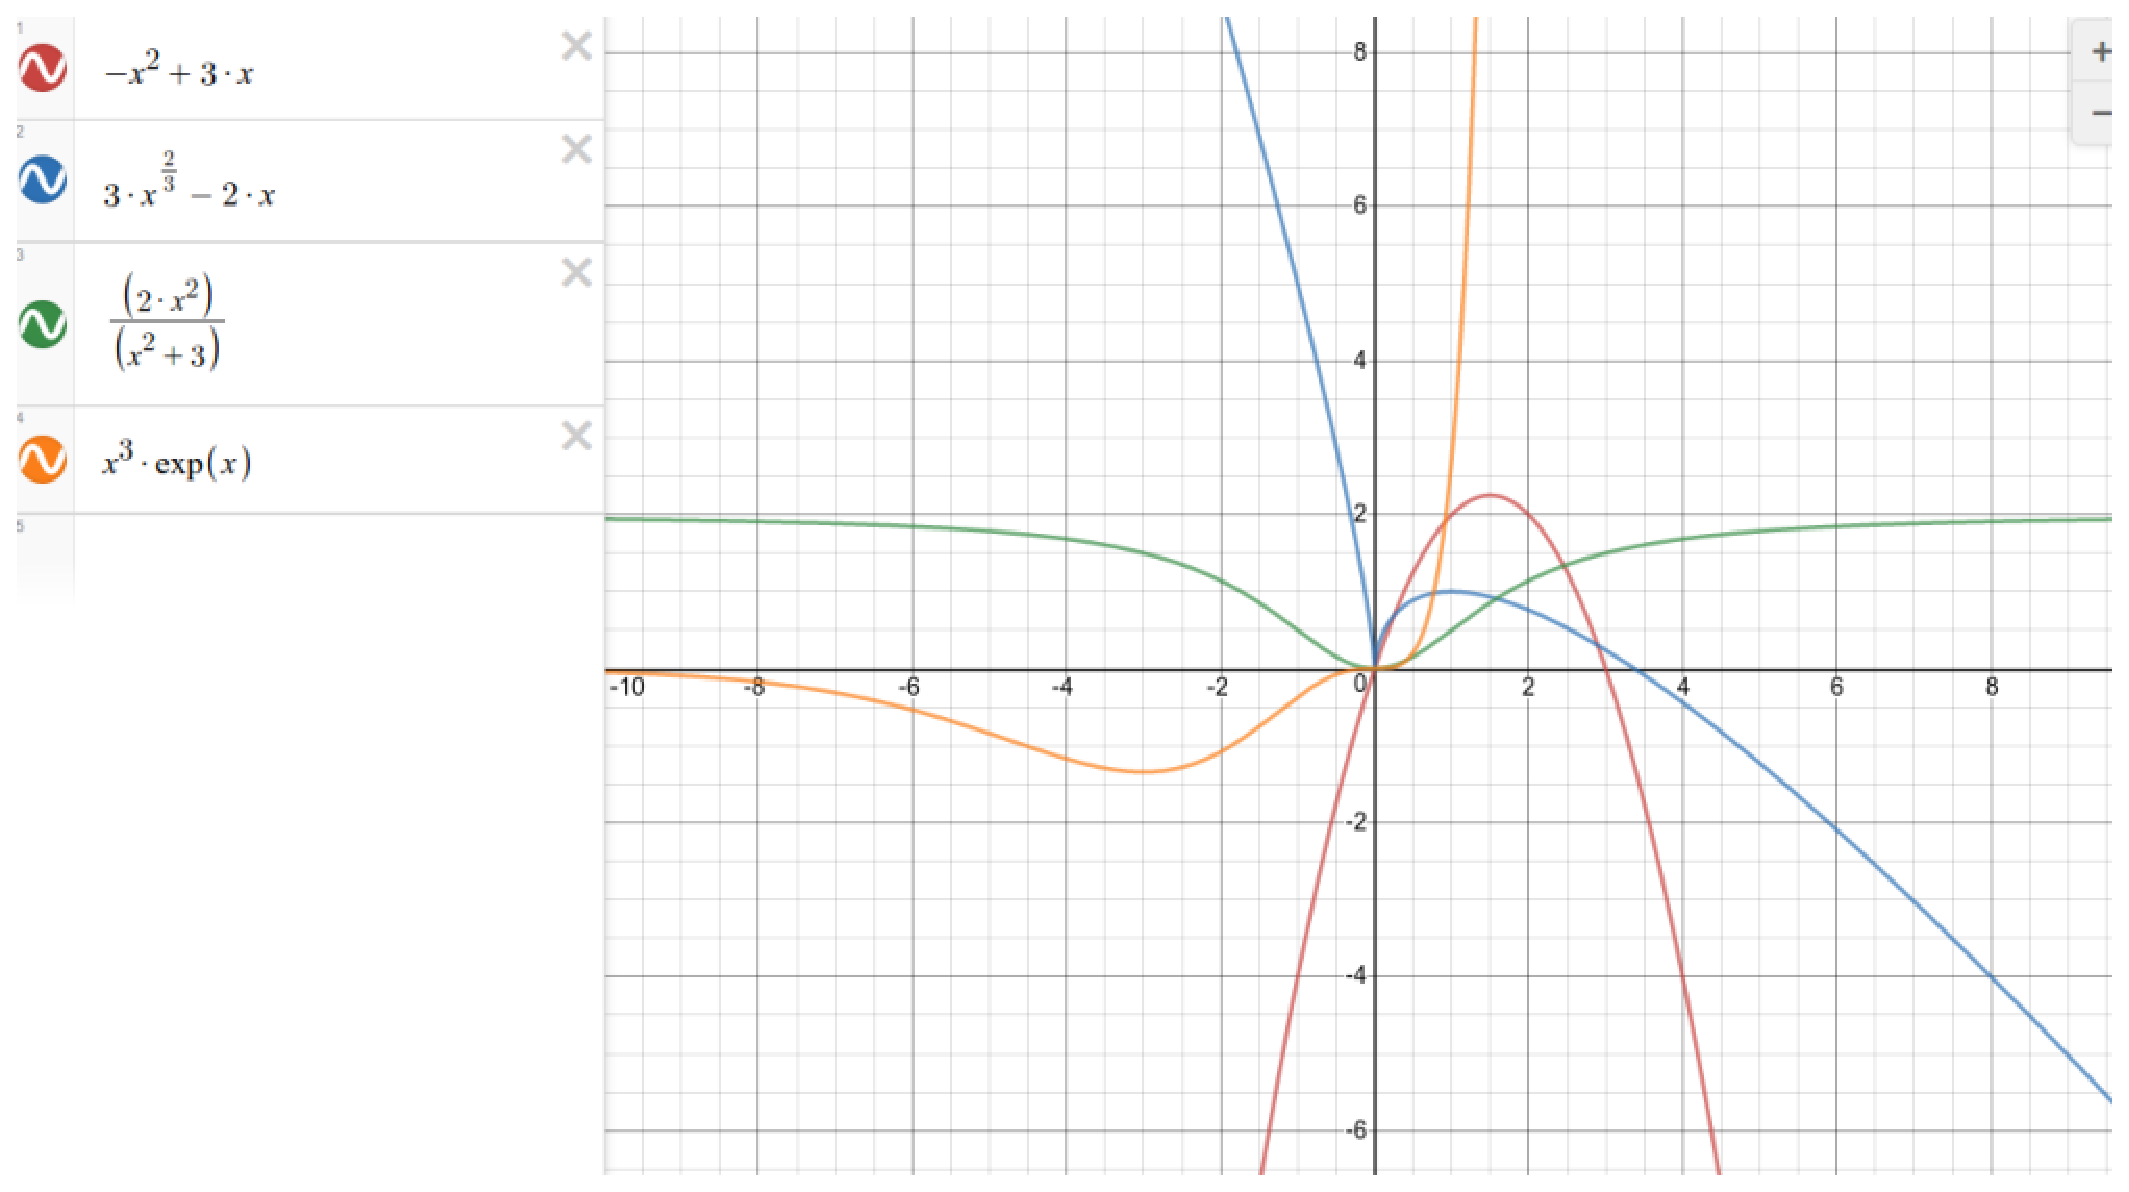
\includegraphics[scale=.4]{./ft-11-AnalyzingFunctions.eps}
  \end{figure}
\end{frame}

\begin{frame}
  \frametitle{End of Lesson}
Next Lesson: Analyzing Functions
\end{frame}

\end{document}

